\documentclass{beamer}


\mode<presentation> {
	\usetheme{Antibes}
	%\setbeamercovered{transparent}
	%\usecolortheme{}
	%\setbeamertemplate{navigation symbols}{ % remove the navigation bar
}

\usepackage{listings}
\usepackage{algorithmic}
\usepackage{algorithm}
\usepackage{amssymb} % symboles mathématiques

\usepackage{listings}
\usepackage[french]{babel}
%\usepackage{beamer}			% problème ???
\usepackage[pdftex]{color}
\usepackage[utf8]{inputenc}
\usepackage{fancybox}

\usepackage{graphicx} % images

\usepackage{pgfpages}			% obsolete ?




\newcommand{\commande}[1]{\fbox{\texttt{\$ #1}}}	% boite
\newcommand{\nbcommande}[1]{\texttt{\$ #1}}					% pas de boite
\newcommand{\multicommande}[1]{
	\framebox[\width]{
	\parbox{\textwidth}{#1}}}


\newcommand{\keyword}[1]{\textbf{\textcolor{blue}{#1}}}
%\newcommand{\code}[1]{\texttt{\textcolor{green}{#1}}}
\newcommand{\code}[1]{\texttt{{#1}}}
\newcommand{\cuda}{\textsc{CUDA}}


%-----------------------------------------------------
%----------------------------------------------------
%---------------------------------------------------
\begin{document}



% possibilites : cf Beamer Tutorial
% Montpellier Singapore Berlin Warsaw Hannover Copenhagen... 
%\usecolortheme{default}

\author{Vincent Barrielle, Simon Cruanes}
\lstset{language=C,showstringspaces=false}	
\title{SAT-solver en \cuda}
\subtitle{projet inf560}



\begin{frame}
\titleframe
\titlepage
\end{frame}

\begin{frame}
\frametitle{Plan}
\small \tableofcontents%[pausesections] 
\normalsize
\end{frame}

%------------------------------------------------
%------------------------------------------------
\section{Algorithme}
%{{{
\begin{frame}
\frametitle{Introduction au problème}
\begin{itemize}
    \item SAT-solving : problème NP-complet dans le cas général
    \pause
    \item Mais important pour l'industrie
    \pause
    \item Algorithmes complets \emph{vs} algorithmes incomplets % TODO
\end{itemize}
\end{frame}

\begin{frame}
\frametitle{DPLL}
\begin{block}{Concept}
\begin{itemize}
    \item Recherche exhaustive classique guidée par une heuristique
    \item \emph{Propagation des clauses unitaires}
\end{itemize}
    \pause
\end{block}

\begin{block}{Remarque}
    Algorithme typiquement récursif $\rightarrow$ non implémentable directement en \cuda.
\end{block}
\end{frame}


\medskip

\begin{algorithm}[h!]
\begin{algorithmic}
\textbf{function} DPLL( $F$ )
  \IF{$F = \emptyset $} 
    \RETURN "Satisfiable"
  \ENDIF
  \STATE $F \gets$ unitPropagation( $F$ )
  \IF{$\square \in F$}  
    \RETURN "not Satisfiable"
  \ENDIF
  \STATE $l \gets$ heuristic( $F$ ) \\
  \RETURN DPLL( $F \cup\{l\}$ ) $\vee$ DPLL( $F \cup \{\lnot l\}$ ) \\

\textbf{function} unitPropagation( $F$ )\\
\WHILE{$\square \not\in F \land \exists $ unit clause $ l \in F$}
  Satisfy $l$ and Simplify $F$ \\
  \RETURN $F$
\ENDWHILE
\end{algorithmic}
\end{algorithm}

\begin{frame}
\frametitle{Implémentation non récursive}

\begin{itemize}
    \item Implémentation basée sur les \keyword{goto} du C
    \item gestion de la pile "à la main"
    \item structures de données optimisées en taille
\end{itemize}
\end{frame}

\begin{frame}
\frametitle{Graphe de flot de contrôle}

\begin{figure}[h]
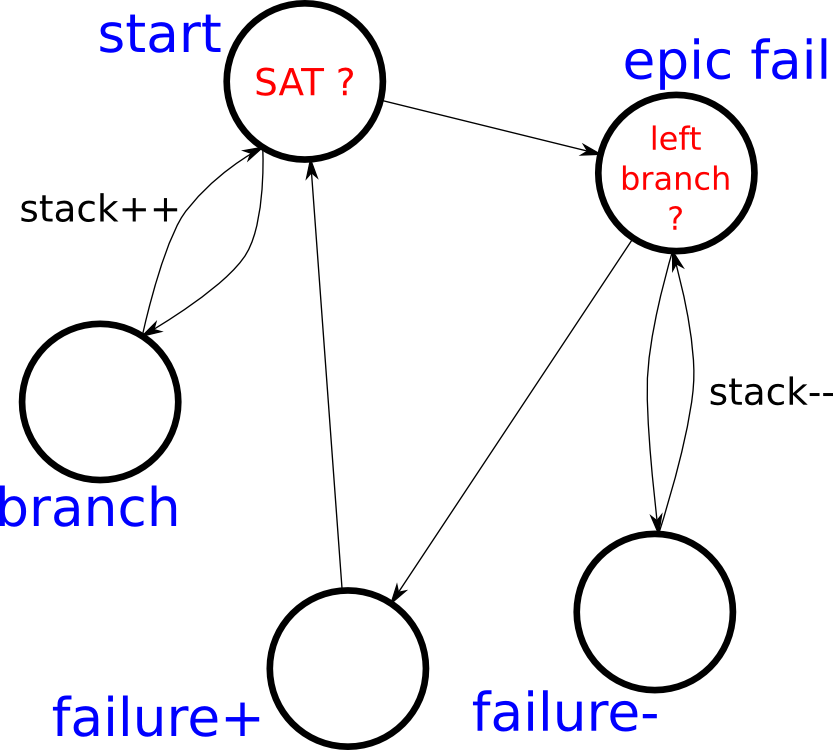
\includegraphics[width = 0.60\textwidth]{control_flow.png}
  \caption[Graphe de flot de controle]{Graphe de flot de contrôle}
\end{figure}

\end{frame}

%}}}


\section{Implémentations parallèles}
%{{{
\begin{frame}
\frametitle{Quelles implémentations ?}

\begin{itemize}
    \item Implémentation mono-threadée, utile pour débugguer et servir de référence
    \pause
    \item Implémentation basée sur \emph{pthreads}
    \pause
    \item Implémentation basée sur \cuda
\end{itemize}
\end{frame}

\begin{frame}
\frametitle{\emph{pthreads}}

\begin{block}{\emph{pthreads}}
\begin{itemize}
    \item threads \textsc{POSIX} de bas niveau
    \item primitives de synchronisation classiques (mutexes, conditions)
\end{itemize}
\end{block}
\pause

\begin{block}{fonctionnement}
\begin{itemize}
    \item lancement avec un nombre quelconque de threads
    \item synchronisation \emph{via} le thread principal
\end{itemize}
\end{block}
\end{frame}



\begin{frame}
\frametitle{\cuda}

\begin{block}{\cuda}
\begin{itemize}
    \item librairie de parallélisme sur cartes graphiques NVidia (GPGPU)
    \item fortes contraintes sur le code (\emph{subset} du C)
\end{itemize}
\end{block}
\pause
\begin{block}{fonctionnement}
\begin{itemize}
    \item lancement de nombreux threads avec des affectations partielles différentes
    \item différence avec les \emph{pthreads} : nombre de coeurs, mais aussi espace mémoire
\end{itemize}
\end{block}
\end{frame}

%}}}

\section{Performances}
%{{{
\begin{block}{remarques générales}
\begin{itemize}
    \item Très faible taille du code $\rightarrow$ tout dans le cache
    \item 0\% de \emph{cache miss} sur les exemples
    \item Grande efficacité de l'implémentation sans récursivité
    \item Mais, pas d'heuristiques très complexes ni de mécanismes complexes
\end{itemize}
\end{block}
\pause

\begin{block}{pthreads}
\begin{itemize}
    \item La version \emph{pthreads} est plus rapide sur les instances satisfiables que la version non concurrente.
    \item Sur les instances non satisfiables, accélération d'un facteur nombre de cœurs.
\end{itemize}
\end{block}

\end{frame}
% TODO : demo
   
%}}}

\section{Difficultés}
%{{{
    
\begin{frame}
\frametitle{difficultés d'implémentations}
\begin{block}{algorithme}
\begin{itemize}
    \item Pas de récursivité ni d'appels de fonction (ni de malloc)
    \item Choix des structures de données
\end{itemize}
\end{block}

\begin{block}{\cuda}
    Mauvaise qualité du compilateur \cuda{}\ldots{}
\end{block}

\end{frame}
%}}}


\end{document}
